% vim: set tw=78 sts=2 sw=2 ts=8 aw et ai:
\documentclass{workshop}

% Comentează liniile de mai jos în cazul în care nu există cod de inclus.
\usepackage{code/highlight}
\usepackage{color}        % dacă e folosit highlight
\usepackage{alltt}        % dacă e folosit highlight

\title[Sesiunea No]{Sesiunea No}
\subtitle{Numele capitolului}
\author{Prenume Nume}
\date{zi lună an}

\begin{document}

% Arătăm numărul frame-ului
\setbeamertemplate{footline}[frame number]

\frame{\titlepage}

% NB: Secțiunile nu sunt marcate vizual, ci doar apar în cuprins
\section{Introducere}

\begin{frame}{Introducere}
  \begin{itemize}
    \item alfa
    \item beta
    \item Extra
      \begin{itemize}
        \item arhaic
        \item proterozoic
      \end{itemize}
  \end{itemize}
\end{frame}

\begin{frame}{Continuare}
  \begin{itemize}
    \item brad
    \item molid
    \item carpen
  \end{itemize}
\end{frame}

\section{Punctul culminant}

\begin{frame}{Problema}
  \begin{columns}
    \pause
    \begin{column}[l]{0.45\textwidth}
      \begin{center}
        Avem un server
      \end{center}
      \begin{figure}
         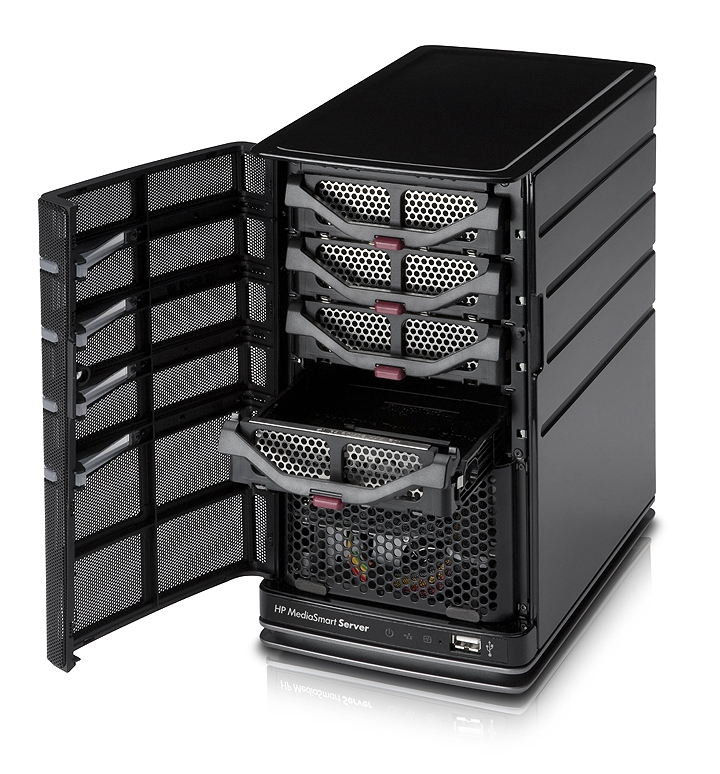
\includegraphics[scale=0.17]{img/hp-server.jpg}
      \end{figure}
    \end{column}
    \pause
    \begin{column}[l]{0.45\textwidth}
      \begin{center}
      Cum procedăm?
      \end{center}
      \begin{figure}
         
\includegraphics[scale=0.25]{img/thinker.jpg}
      \end{figure}
    \end{column}
  \end{columns}
\end{frame}

\begin{frame}[fragile]{Cod verbatim}
  \pause
  \footnotesize
  \begin{verbatim}
brw-rw----  1 root disk      8,   0 Oct  2 21:53 sda
brw-rw----  1 root disk      8,   1 Oct  2 21:53 sda1
brw-rw----  1 root disk      8,  10 Oct  2 18:53 sda10
brw-rw----  1 root disk      8,  11 Oct  2 21:53 sda11
crw-rw----  1 root root      4,   0 Oct  2 21:53 tty0
crw-rw----  1 root root      4,  10 Oct  2 21:53 tty10
crw-rw----  1 root root      4,  11 Oct  2 21:53 tty11
crw-rw----  1 root root      4,  12 Oct  2 21:53 tty12
  \end{verbatim}
\end{frame}

\begin{frame}{Informații de stare}
  \input{code/user-stat}
\end{frame}

\section{Keywords}

\begin{frame}{Cuvinte cheie}
  \begin{columns}
    \begin{column}[l]{0.5\textwidth}
      \begin{itemize}
        \item certificări
        \item LPIC
        \item GNU/Linux
        \item Debian
        \item sysfs
        \item procfs
        \item udev
        \item dispozitive
      \end{itemize}
    \end{column}
    \begin{column}[l]{0.5\textwidth}
      \begin{itemize}
        \item apropos, man, info
        \item linie de comandă
        \item shell
        \item biblioteca readline
        \item pachete, PMS
        \item dpkg, apt
        \item utilizatori, grupuri
        \item parole
      \end{itemize}
    \end{column}
  \end{columns}
\end{frame}

\begin{frame}{Resurse utile}
  \begin{itemize}
    \item James Turnbull, Peter Lieverdink, Dennis Matotek -- Pro Linux System
    Administration
    \item \url{http://elf.cs.pub.ro/pisr/}
    \item
    \url{http://www.lpi.org/index.php/eng/certification/the_lpic_program}
    \item \url{http://debian.org/doc/user-manuals}
    \item \url{http://wiki.debian.org/}
    \item \url{http://www.debian-administration.org/}
  \end{itemize}
\end{frame}

\section{Întrebări}

\end{document}
